\documentclass{beamer}
%\documentclass[xcolor=dvipsnames]{beamer}
\usepackage[spanish]{babel}
\usepackage[utf8]{inputenc}
\usepackage{graphicx}
\usepackage{latexsym}

\newcommand{\beamer}{\textsc{beamer}}
\newtheorem{definicion}{Definición}
\newtheorem{ejemplo}{Ejemplo}

%%%%%%%%%%%%%%%%%%%%%%%%%%%%%%%%%%%%%%%%%%%%%%%%%%%%%%%%%%%%%%%%%%%%%%%%%%%%%%%
\title[Trabajo de Fin de Máster]{Sistemas y Tecnologías Web Aplicadas\\
Shell para corrección automática de repositorios de GitHub}

\author[Juan José Labrador González] {
Autor: Juan José Labrador González \\
Director: Casiano Rodríguez León
}

\institute[ULL]{Escuela Superior de Ingeniería y Tecnología \\
                Departamento de Ingeniería Informática y de Sistemas \\
                Universidad de La Laguna}
\date[14-07-2017]{14 de julio de 2017}
%%%%%%%%%%%%%%%%%%%%%%%%%%%%%%%%%%%%%%%%%%%%%%%%%%%%%%%%%%%%%%%%%%%%%%%%%%%%%%%

%\usetheme{Berlin}
\usetheme{Madrid}

%%%%%%%%%%%%%%%%%%%%%%%%%%%%%%%%%%%%%%%%%%%%%%%%%%%%%%%%%%%%%%%%%%%%%%%%%%%%%%%
\definecolor{pantone254}{RGB}{122,59,122}
\definecolor{pantone3015}{RGB}{0,88,147}
\definecolor{pantone432}{RGB}{56,61,66}
\setbeamercolor*{palette primary}{use=structure,fg=white,bg=pantone254}
\setbeamercolor*{palette secondary}{use=structure,fg=white,bg=pantone3015}
\setbeamercolor*{palette tertiary}{use=structure,fg=white,bg=pantone432}
\setbeamercolor*{palette sidebar primary}{use=structure,fg=pantone254}
\setbeamercolor*{palette sidebar tertiary}{use=structure,fg=pantone3015}
\setbeamercolor*{block title}{bg=pantone3015,fg=white}
\setbeamercolor*{alerted text}{fg=pantone432}
\setbeamercolor*{item projected}{fg=pantone254}
\setbeamercolor*{section in toc shaded}{use=structure,fg=structure.fg}
\setbeamercolor*{section in toc}{fg=pantone3015}
\setbeamercolor*{subsection in toc shaded}{fg=pantone3015}
\setbeamercolor*{subsection in toc}{fg=pantone432}

%%%%%%%%%%%%%%%%%%%%%%%%%%%%%%%%%%%%%%%%%%%%%%%%%%%%%%%%%%%%%%%%%%%%%%%%%%%%%%%
\begin{document}
  
%++++++++++++++++++++++++++++++++++++++++++++++++++++++++++++++++++++++++++++++  
\begin{frame}

  \includegraphics[width=0.15\textwidth]{images/ullesc.eps}
  \hspace*{7.5cm}
  \includegraphics[width=0.16\textwidth]{images/etsii.eps}
  \titlepage

\end{frame}
%++++++++++++++++++++++++++++++++++++++++++++++++++++++++++++++++++++++++++++++  

%++++++++++++++++++++++++++++++++++++++++++++++++++++++++++++++++++++++++++++++  
\begin{frame}
  \frametitle{Índice}  
  \tableofcontents
\end{frame}
%++++++++++++++++++++++++++++++++++++++++++++++++++++++++++++++++++++++++++++++  

\section{Introducción}
\begin{frame}[fragile]
  \frametitle{Introducción}
  
  	\begin{center}
    	Este Trabajo de Fin de Máster consistió en la creación de una herramienta de línea de comandos que permite la automatización de tareas sobre repositorios de GitHub.
    \end{center} 
    \bigskip
    
    \underline{{\bfseries Características}}:
    
    \begin{columns}
        % First column
        \begin{column}{9cm}
        	\begin{itemize}
	        	\item Escrita en {\bfseries Node.js}
    		    \item Distribuida mediante un {\bfseries paquete NPM}.
	    	   	\item Multiplataforma: Linux, macOS, Windows.
	       		\item Uso sencillo.
	       	\end{itemize}
        \end{column}
        % Second column
        \begin{column}{8cm}
          
\includegraphics[width=0.4\textwidth]{images/cross_platform.eps}
        \end{column}
      \end{columns}
   
\end{frame}
  %+++++++++++++++++++++++++++++++++++++++++++++++++++++++++++++++++++++++++++++++++++++++++++++++++++++++++++++++++++++++++++++++++++++++++++
 
\section{Estado del arte y motivación}
\begin{frame}[allowframebreaks]
	\frametitle{Estado del arte y motivación}
	
	\underline{{\bfseries Sistemas de Control de Versiones}}
	\bigskip
	
	\begin{itemize}
       \item Indispensables en la Ingeniería del Software.
	   \item Constante crecimiento en número y funcionalidades. 
	   \item Fomento de la colaboración.	
	\end{itemize}
	\bigskip
	
	\begin{center}
		
\includegraphics[width=0.6\textwidth]{images/control-versiones2.eps}
	\end{center}
	
	\framebreak
	%-------------------------------------

	\vspace*{0.18cm}	
	\underline{{\bfseries GitHub}}

	\begin{itemize}
       \item Plataforma de desarrollo colaborativo consolidada.
       \begin{center}
	       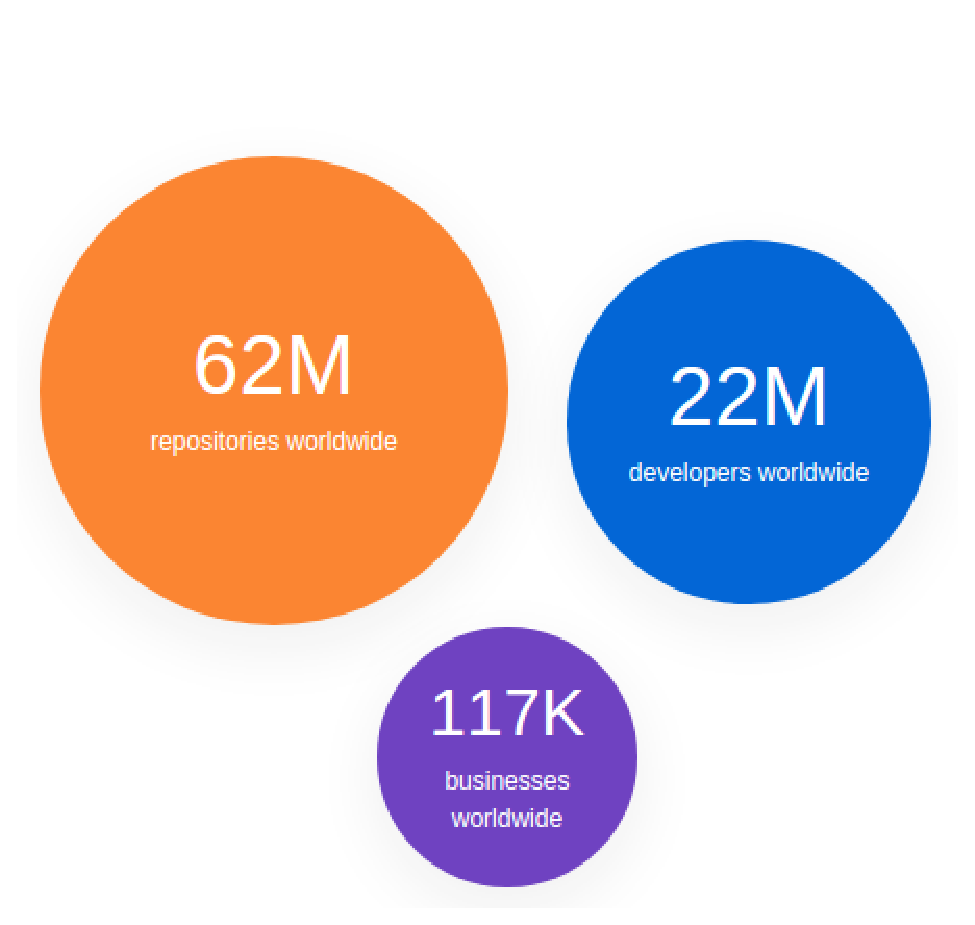
\includegraphics[width=0.5\textwidth]{images/github-stats.eps}
	   \end{center}
       \framebreak
       %-------------------------------------
       
       \item Usa {\bfseries Git} como sistema de control de versiones.        
	   \item Fuerte apuesta por la educación:
	   \bigskip
	   
	   	\begin{columns}
        	% First column
        	\begin{column}{4.5cm}
        		\includegraphics[width=1.2\textwidth]{images/github-sdp.eps}
        	\end{column}
        	% Second column
        	\begin{column}{3.5cm}
          		
\includegraphics[width=1.2\textwidth]{images/github-classroom.eps}
        	\end{column}
      	\end{columns}
	\end{itemize}
	\framebreak
	%-------------------------------------
	
	\underline{{\bfseries Motivación}} 
	\bigskip
	
	\begin{itemize}
       \item Imposibilidad de realizar operaciones masivas sobre repositorios.
	   \item Ausencia de herramientas externas para tal fin.
	   \item Mejor aprovechamiento de las herramientas educativas.
	   \item Simplificación del trabajo del docente.
	   \item Ahorro considerable de tiempo en tareas repetitivas.
	\end{itemize}
	\framebreak
	%-------------------------------------
	
	\underline{{\bfseries Ejemplo de caso real}}
	\bigskip
	
	\begin{itemize}
       \item Asignatura cuatrimestral con 10 prácticas evaluables.
	   \item Total de alumnos matriculados: 50.
	   \item Total de prácticas por alumno: 10.
	\end{itemize}
	
	\begin{center}
		$10 \times 50$ = {\bfseries 500 repositorios}
	\end{center}
	\begin{center}
		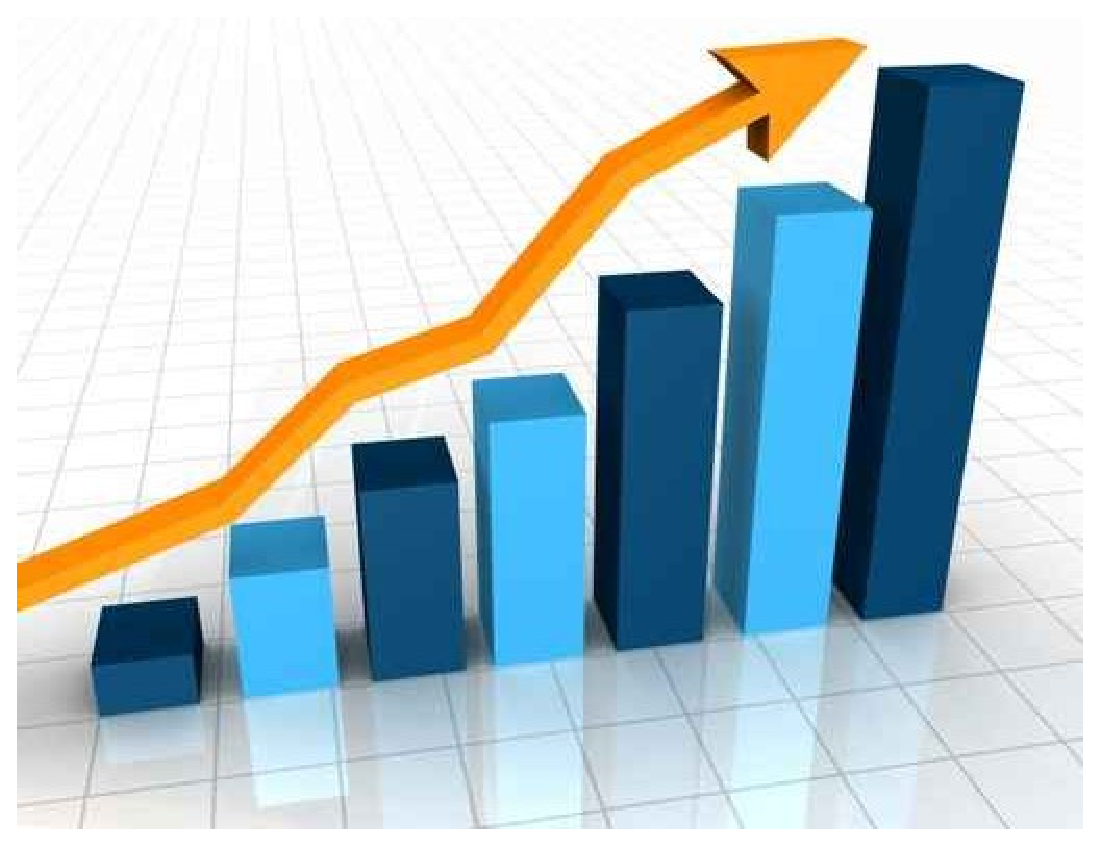
\includegraphics[width=0.3\textwidth]{images/grafico-ascendente.eps}	
	\end{center}
	
\end{frame}
  %+++++++++++++++++++++++++++++++++++++++++++++++++++++++++++++++++++++++++++++++++++++++++++++++++++++++++++++++++++++++++++++++++++++++++++
  
\section{Perfil de Usuario}
\begin{frame}
  \frametitle{Perfil de Usuario}
  La herramienta desarrollada está principalmente orientada hacia un perfil de profesor concreto:
  \bigskip
    
  \begin{itemize}
	\item Docente de alguna rama de Ingeniería Informática.
	\item Con conocimientos avanzados en:
	\begin{itemize}
		\item Programación.
		\item Herramientas de control de versiones.
	\end{itemize}
  \end{itemize}
  
  \begin{center}
		
\includegraphics[width=0.7\textwidth]{images/technologies.eps}	
	\end{center}

\end{frame}
%++++++++++++++++++++++++++++++++++++++++++++++++++++++++++++++++++++++++++++++  

\section{Objetivos}
\begin{frame}
  \frametitle{Objetivos}
  
  %Los objetivos que se han propuesto a completar han sido los siguientes:
  \begin{columns}
    % First column
    \begin{column}{9cm}
      \begin{itemize}
        \item Revisión biliográfica y consulta del estado del arte.
        \item Desarrollo de una herramienta de línea de comandos escrita en {\bfseries Node.js} que permita: 
        \begin{itemize}
          \item Autenticación de usuarios.
          \item Listar organizaciones, asignaciones y repositorios del usuario.
          \item Automatizar la descarga de repositorios y la ejecución de scripts en los mismos:
          \begin{itemize}
             \item TDD.
             \item Creación de entorno.
             \item Evaluación.
          \end{itemize}
          \item Presentación de resultados al usuario:
          \begin{itemize}
             \item PDF.
             \item HTML.
          \end{itemize}
        \end{itemize}
      \end{itemize}
    \end{column}
    % Second column
    \begin{column}{5cm}
      
\includegraphics[width=0.7\textwidth]{images/checklist.eps}
    \end{column}
  \end{columns}
  
\end{frame}

%++++++++++++++++++++++++++++++++++++++++++++++++++++++++++++++++++++++++++++++  

\section{Tecnología usada}
\begin{frame}
  \frametitle{Tecnología usada}
  
  \begin{center}
  	
\includegraphics[width=0.45\textwidth]{images/nodejs-logo.eps}
  
  
  	%\begin{columns}
        	% First column
     %   	\begin{column}{4cm}
        		
\includegraphics[width=0.32\textwidth]{images/npm.eps}
        		\hspace*{1cm}
      %  	\end{column}
        	% Second column
       % 	\begin{column}{2cm}
          		\includegraphics[width=0.17\textwidth]{images/github.eps}
          		        		\hspace*{0.3cm}
        %	\end{column}
        %	\begin{column}{4cm}
          		
\includegraphics[width=0.45\textwidth]{images/travis-ci-logo.eps}
        %	\end{column}
      	%\end{columns} 
  \end{center}
  
	 
  

\end{frame}

%++++++++++++++++++++++++++++++++++++++++++++++++++++++++++++++++++++++++++++++  

\section{Metodología de desarrollo}
\begin{frame}[allowframebreaks]
  \frametitle{Metodología de desarrollo}
  
  Metodología {\bfseries ágil}:
  \begin{itemize}
    \item Reuniones periódicas estableciendo iteraciones cortas.
    \item Desarrollo y presentación de resultados y prototipos tras cada iteración.
    \item Solución de problemas e incorporación de nuevas características. 
  \end{itemize}
  \framebreak
    
  
  \begin{columns}
    % First column
    \begin{column}{5cm}
    	{\bfseries GitHub}
      \begin{itemize}
        \item Control de versiones usando \textit{branching}.
        \item Gestión de incidencias y mejoras usando \textit{issues}.
      \end{itemize}
      
\includegraphics[width=0.5\textwidth]{images/octocat.eps}
    \end{column}
    % Second column
    \begin{column}{5cm}
    {\bfseries Travis-CI}
    \begin{itemize}
        \item Control de despliegues.
      \end{itemize}

        
\includegraphics[width=0.7\textwidth]{images/travis-ci-logo.eps}

    \end{column}
  \end{columns}
  
\end{frame}

%++++++++++++++++++++++++++++++++++++++++++++++++++++++++++++++++++++++++++++++

\section{Resultados}
\begin{frame}
\frametitle{Resultados}
  
  \begin{center}
    \Huge{Resultados}
  \end{center}
\end{frame}

\subsection{Funcionalidades requeridas}
\begin{frame}
\frametitle{Funcionalidades requeridas}
  \bigskip
  \bigskip
  
  \begin{itemize}
    \item Autenticación con GitHub
    \item Listar organizaciones, asignaciones y repositorios de GitHub del usuario
    \item Automatizar la descarga de repositorios
    \item Automatizar la ejecución de scripts en los repositorios
    \item Recopilar y presentar la información obtenida de la automatización de tareas
  \end{itemize}
  
  
\end{frame}
  %+++++++++++++++++++++++++++++++++++++++++++++++++++++++++++++++++++++++++++++++++++++++++++++++++++++++++
  
\subsection{Funcionalidades extra}
  
\begin{frame}[allowframebreaks]
\frametitle{Funcionalidades extra}
  Funcionalidades que, a pesar de no ser requeridas, brindan al usuario de una mejor experiencia de uso del programa:
  \bigskip
  
  \begin{itemize}
    \item Autocompletado de los comandos.
    Pull Request.
    \item Opción de ayuda.
    \item Opción de visualizar el directorio de trabajo actual
    \item Opción para conocer el propietario de cada repositorio
    \framebreak
    %+++++++++++++++++++++++++++++++++++++++++++++++++++++++++++++++++++++++++++++++++++++++++
    
  \end{itemize}  
\end{frame}

%++++++++++++++++++++++++++++++++++++++++++++++++++++++++++++++++++++++++++++++  

\section{Conclusiones y Trabajos Futuros/Conclusions and Future Work}
\begin{frame}[allowframebreaks]
  \frametitle{Conclusiones y Trabajos Futuros/Conclusions and Future Work}
  
  \begin{itemize}
    \item Esta herramienta pretende ser un complemento para....
    \item a
    \item a
  \end{itemize}
  \framebreak
  %+++++++++++++++++++++++++++++++++++++++++++++++++++++++++++++++++++++++++++++++++++++++++++++++++++++++++++++++++++++++++++++++++++++++++++
  
  {\bf Trabajos Futuros:}
  \begin{itemize}
    \item Generar scripts en Bash para evaluar aplicaciones (instalación de dependencias, comprobación de calidad de código y ejecución de tests) en varios lenguajes: Node.js, C++, Ruby, Python, etc.
    \item Dar soporte a la ejecución de scripts escritos en otros lenguajes: Ruby, Python...
    \item Generar issues en cada repositorio con los resultados de los scripts que se ejecuten.
    \item Crear ramas en cada repositorio con los resultados de los scripts.
  \end{itemize}
  \framebreak
  %+++++++++++++++++++++++++++++++++++++++++++++++++++++++++++++++++++++++++++++++++++++++++++++++++++++++++++++++++++++++++++++++++++++++++++
  
  \begin{itemize}
    \item This tool intends to ...
    \item It uses ....
    \item On the other hand...
  \end{itemize}
  \framebreak
  %+++++++++++++++++++++++++++++++++++++++++++++++++++++++++++++++++++++++++++++++++++++++++++++++++++++++++++++++++++++++++++++++++++++++++++
  
  {\bf Future Work:}
  \begin{itemize}
    \item a
    \item a
    \item a
    \item a
  \end{itemize}
\end{frame}

%++++++++++++++++++++++++++++++++++++++++++++++++++++++++++++++++++++++++++++++ 

\section{Bibliografía}
\begin{frame}[allowframebreaks]
  \frametitle{Bibliografía}
  \bibliographystyle{ieeetr}
  \bibliography{presentacion_tfm}
  \nocite{*}
\end{frame}

\begin{frame}
  \frametitle{Fin de la presentación}
  \begin{center}
    \Huge{Gracias por su atención}
  \end{center}
\end{frame}

\end{document}
